\subsection{Development}\label{sec:development}
\subsubsection{Tools}
While designing the project, I used low-fidelity, analog tools to quickly generate ideas and gather feedback on them, beginning with paper- and whiteboard sketches. I used the Pencil Prototyping tool\footnote{\url{http://pencil.evolus.vn/Next.html}} to create wireframes for another round of feedback. I then constructed the actual webpage and visualizations using the D3.js JavaScript library\footnote{\url{https://d3js.org/}} for the visualizations and HTML5/CSS3 for the page layout. The page display conforms to responsive web design principles, although the interactive aspects of the visualizations do not.

\subsubsection{Process}
As discussed above, the project began as a series of conceptual sketches, which allowed me to quickly try out ideas and revise them to find an appropriate design. \autoref{fig:whiteboard} shows some of these early sketches, featuring ideas for page layout, navigation, and transitional animations. They also include my annotations of feedback I received: while I discuss user evaluations in \autoref{sec:testing}, testing began at this stage and continued throughout the project.

\begin{figure}
  \begin{minipage}{0.5\textwidth}
    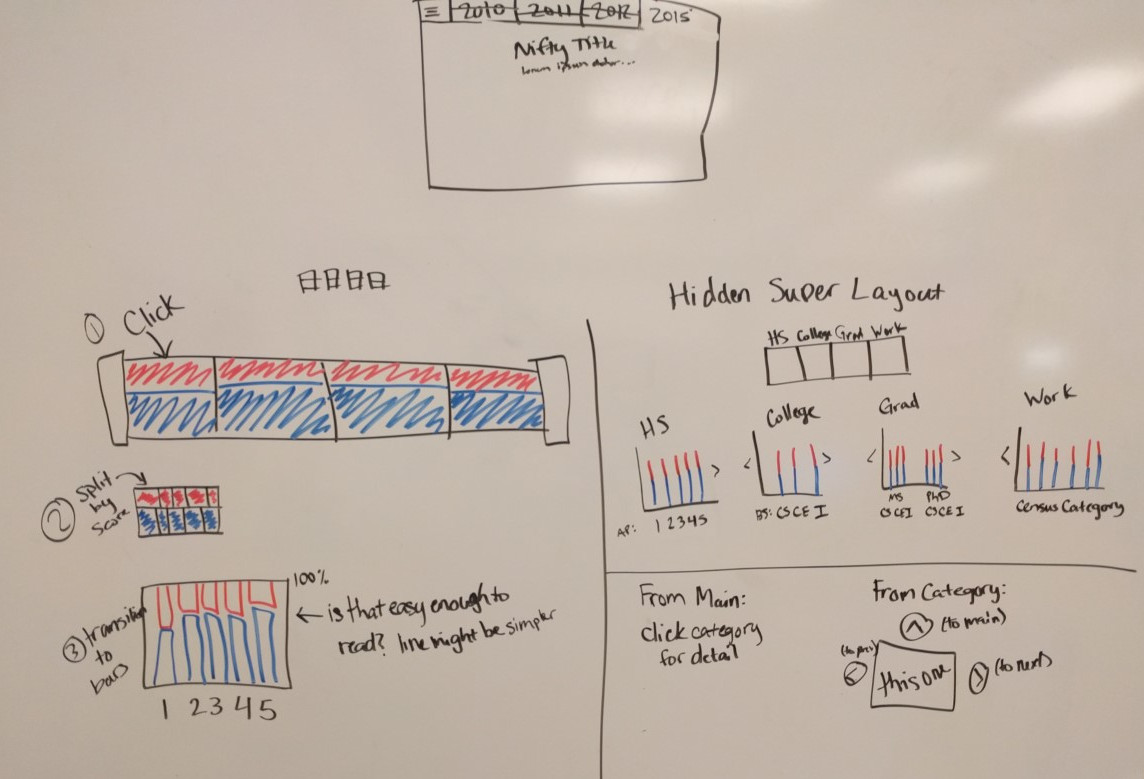
\includegraphics[width=\textwidth]{whiteboard-1-layout}
  \end{minipage}
  \begin{minipage}{0.5\textwidth}
    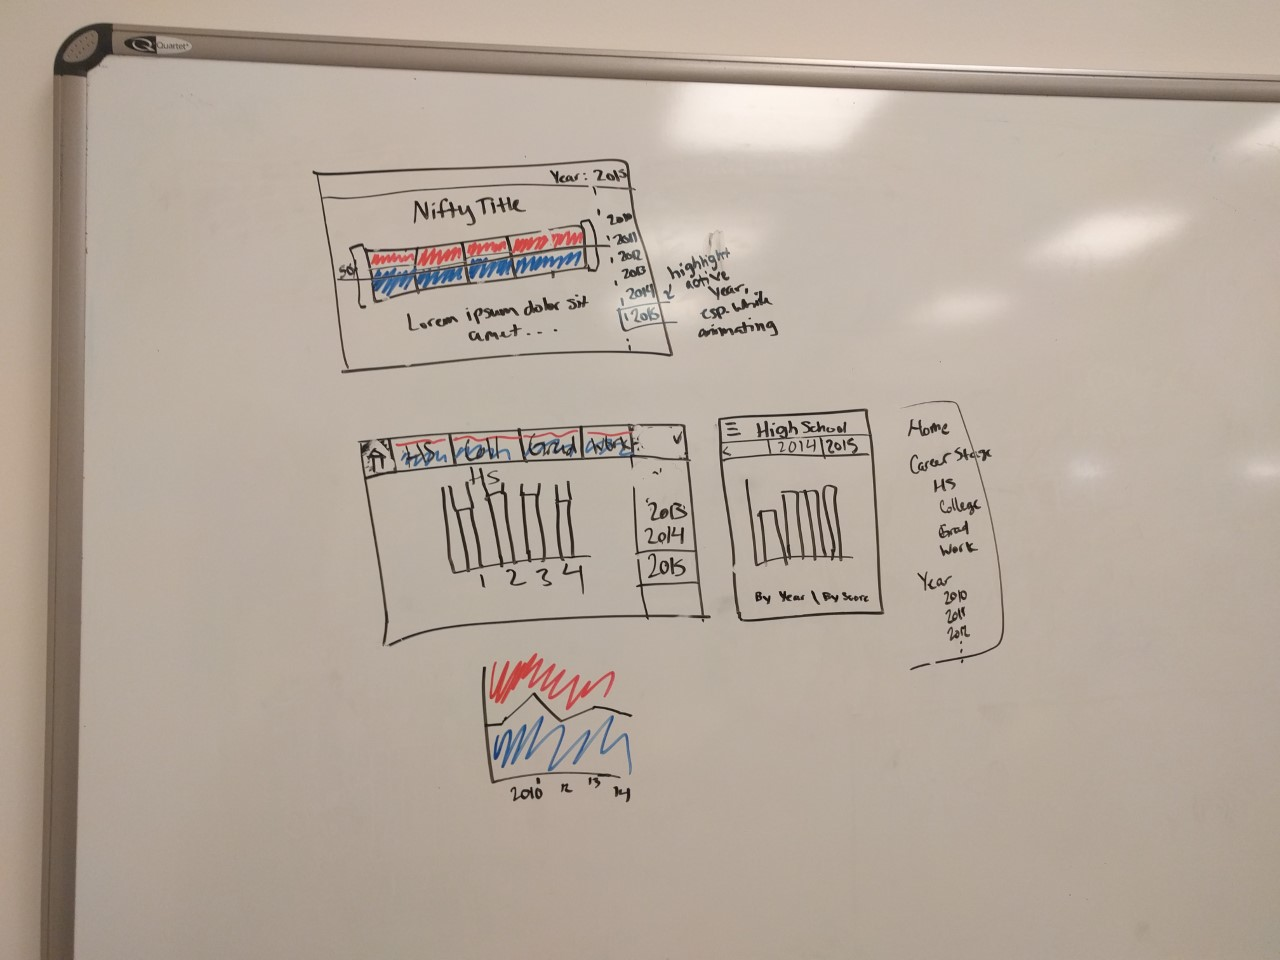
\includegraphics[width=\textwidth]{whiteboard-2-navigation}
  \end{minipage}
  \caption{Early Design Sketches: data display (left) and page navigation (right)}\label{fig:whiteboard}
\end{figure}

Considering my design goals in light of that initial feedback, I decided to focus on a simple data display that is easy for a general audience to interpret. The page begins with an overview of the entire pipeline, allowing users to see all of the high-level data at once; scrolling down reveals detailed views of each stage in the pipeline. This detail view includes two bar graphs: one showing the demographic breakdown for each year of data, and one showing the number of men and women in each subgroup (degree program, occupation, or exam score). Each of those detailed views employs the same structure, so that users learn from earlier graphs how to read and interact with the later ones. A short paragraph accompanying each graph directs viewers to points of interest within that stage. \autoref{fig:wireframe} shows wireframes of the overview and details panel.

\begin{figure}
  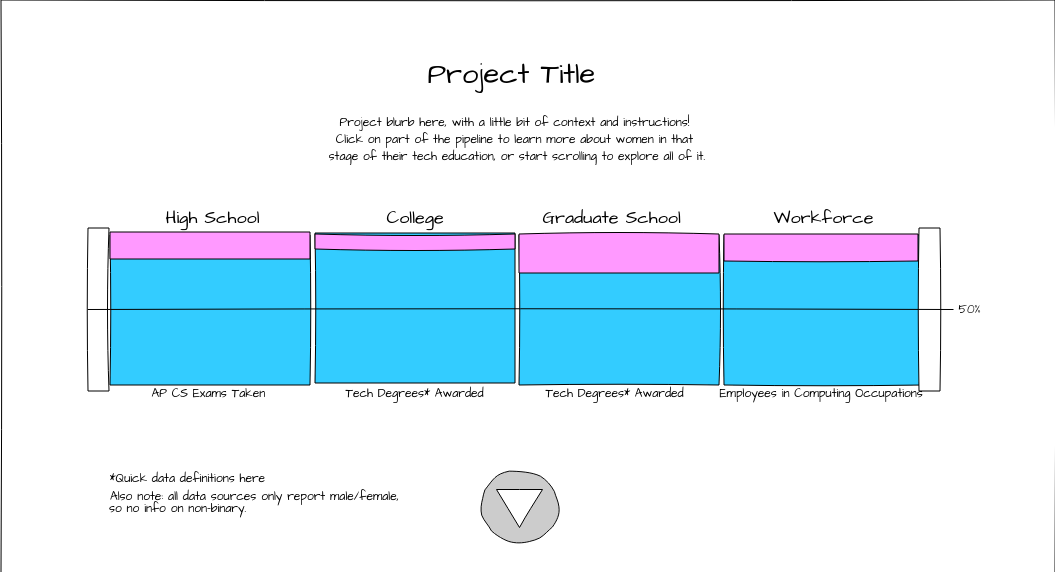
\includegraphics[width=\textwidth]{wireframe-1-overview}

  \vspace{2cm}

  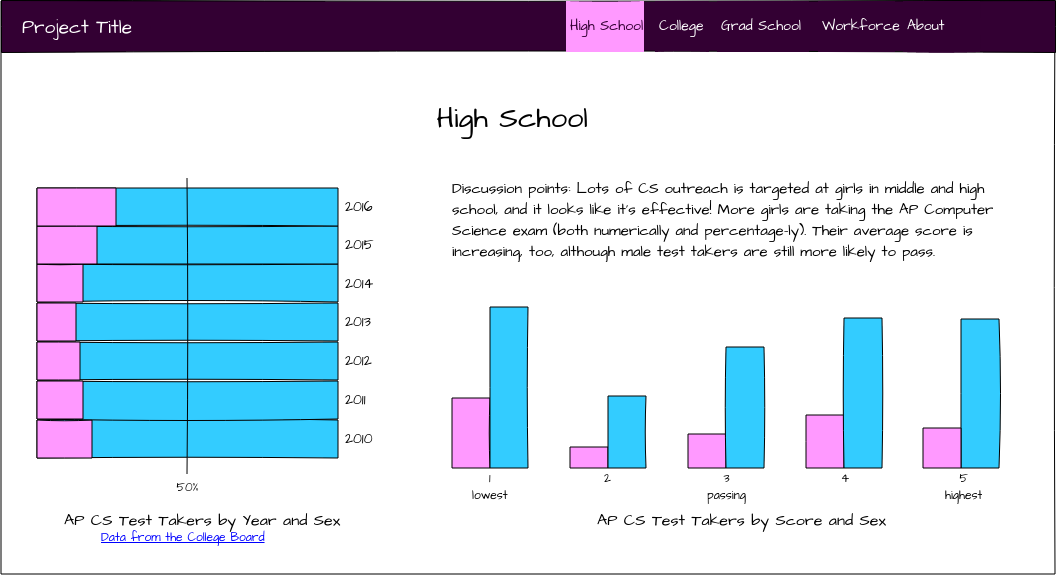
\includegraphics[width=\textwidth]{wireframe-2-hs-detail}
  \caption{Wireframes: overview (top) and high school detail (bottom)}\label{fig:wireframe}
\end{figure}

The completed webpage, shown in \autoref{fig:screenshot}, follows essentially the same structure, adding narrative interludes between each of the detailed views to provide context without cluttering the data views. Hovering over each graph gives users a dark reference line and a numerical indicator of the percentage of women at that point on the graph, as seen in the bottom view of \autoref{fig:screenshot}.

\begin{figure}
  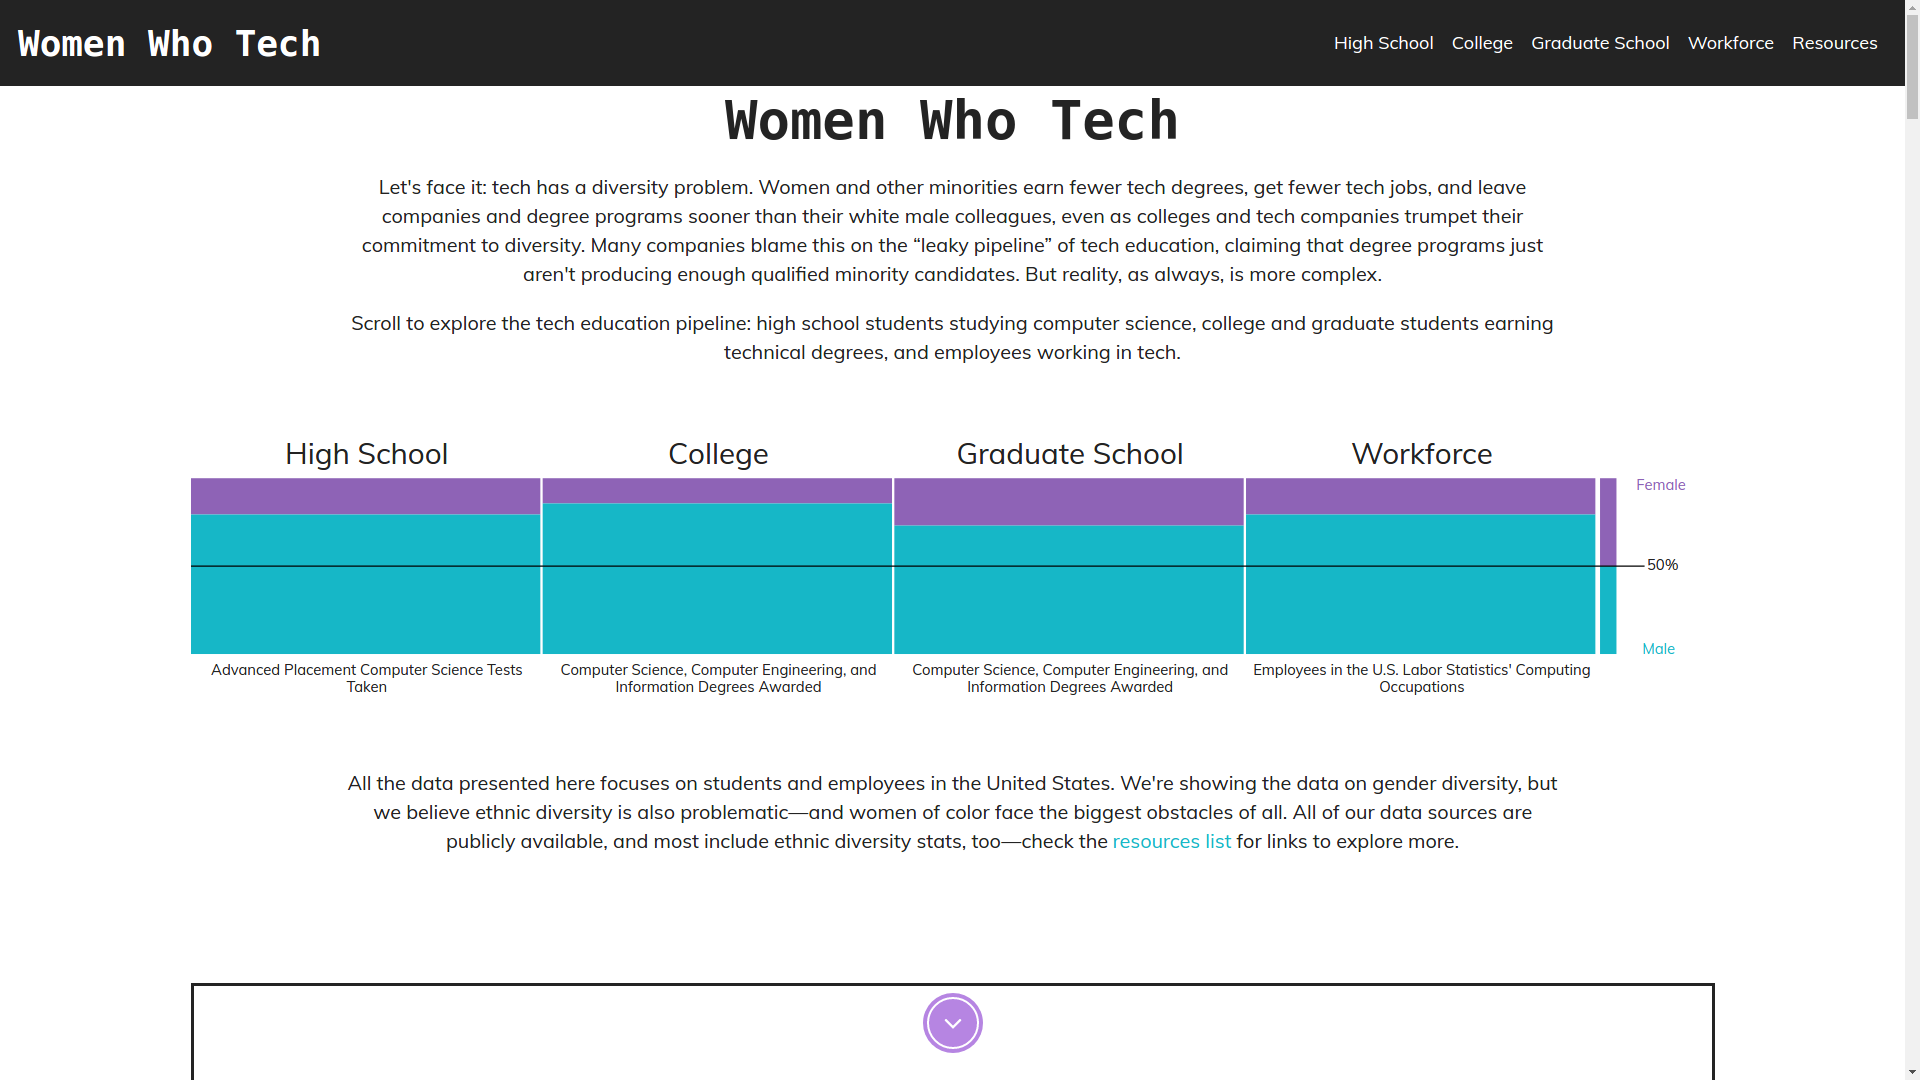
\includegraphics[width=0.95\textwidth]{screen-1-overview}


  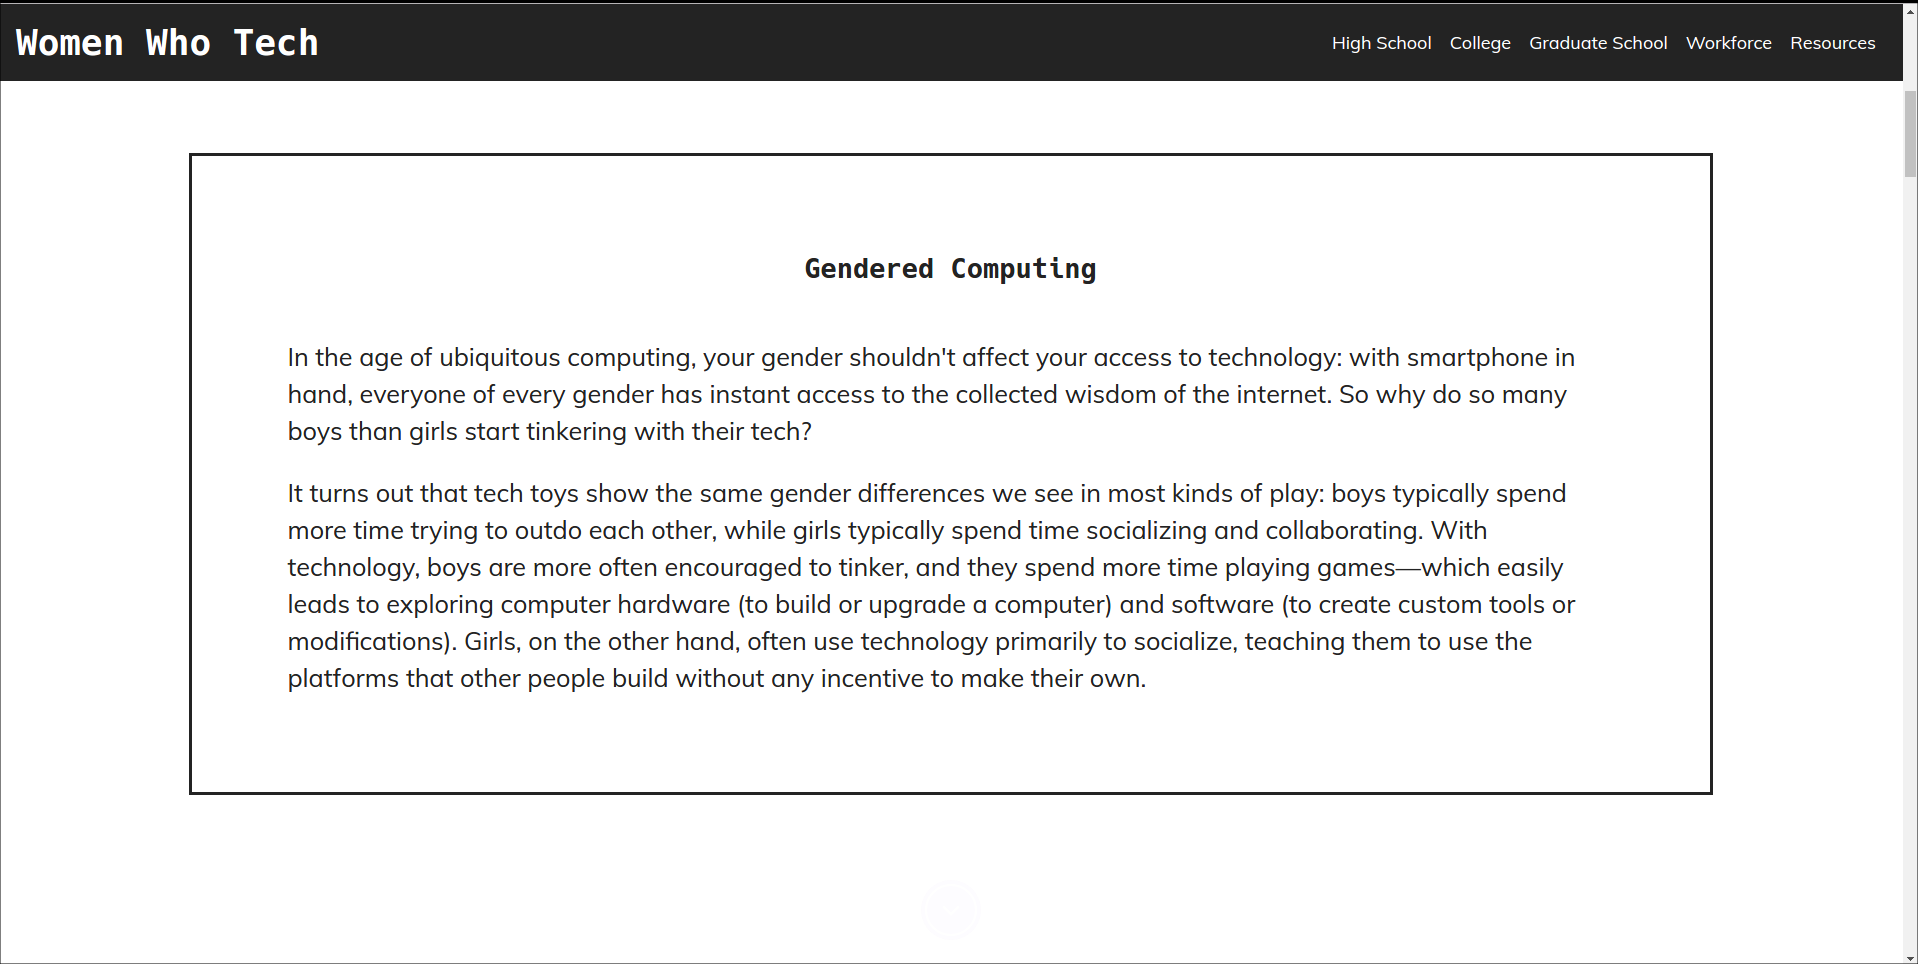
\includegraphics[width=0.95\textwidth]{screen-2-interlude}


  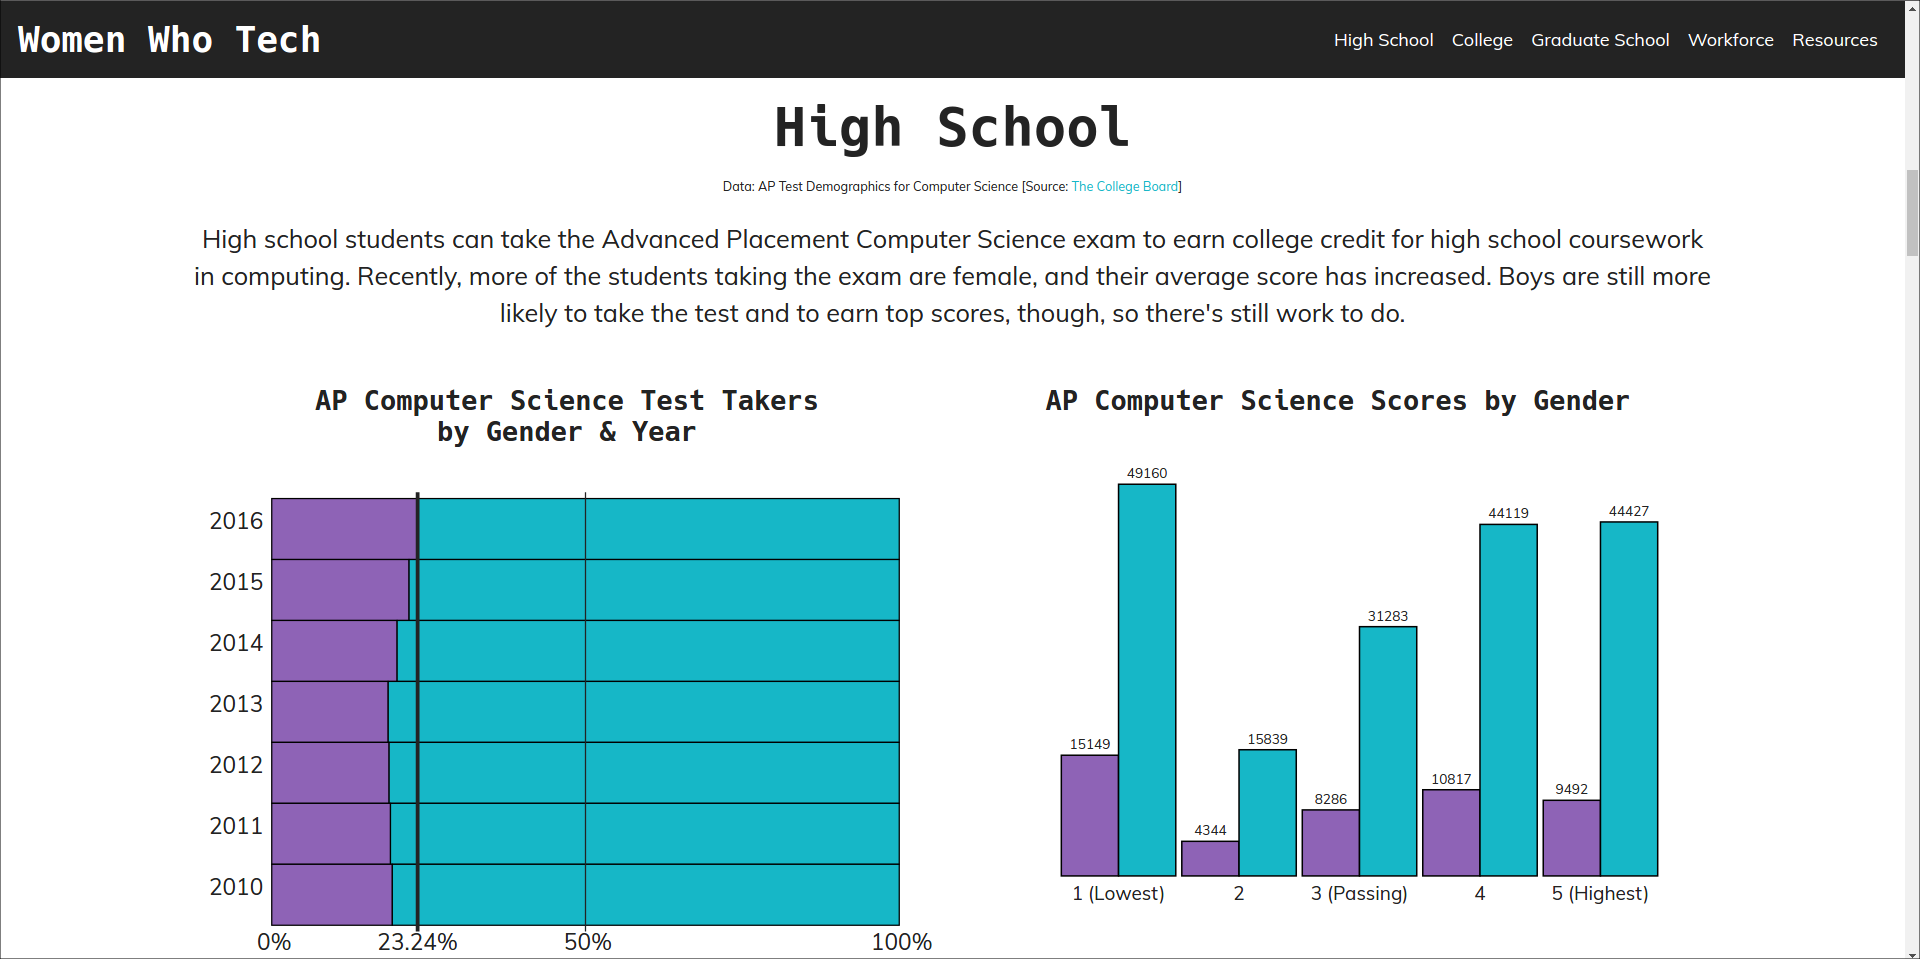
\includegraphics[width=0.95\textwidth]{screen-3-hs-detail}
  \caption{Screenshots: overview (top), narrative frame (middle), and high school detail (bottom)}\label{fig:screenshot}
\end{figure}
